% Made up for the tikra benchmark.
\usetikzlibrary{shapes.geometric}
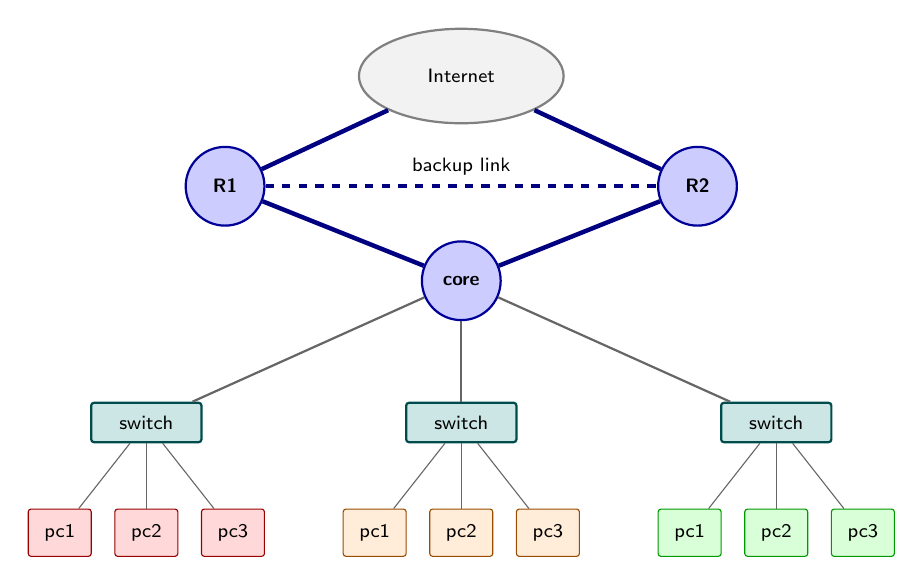
\begin{tikzpicture}[font=\sffamily\scriptsize,
    router/.style={circle, draw=blue!60!black, fill=blue!20, thick, minimum size=1cm, font=\sffamily\bfseries\scriptsize},
    switch/.style={rectangle, draw=teal!60!black, fill=teal!20, thick, minimum width=1.4cm, minimum height=5mm, rounded corners=1pt},
    host/.style={rectangle, minimum width=8mm, minimum height=6mm, rounded corners=1pt},
    cloud/.style={ellipse, draw=gray, fill=gray!10, thick, minimum width=2.6cm, minimum height=1.2cm},
    link/.style={thick, black!60},
    wan/.style={ultra thick, blue!50!black}]
  \node[cloud] (net) at (0,3) {Internet};
  \node[router] (r1) at (-3,1.6) {R1};
  \node[router] (r2) at (3,1.6) {R2};
  \node[router] (core) at (0,0.4) {core};
  \draw[wan] (net) -- (r1); \draw[wan] (net) -- (r2);
  \draw[wan] (r1) -- (core) -- (r2);
  \draw[wan, dashed] (r1) -- node[above, black] {backup link} (r2);
  \foreach \s/\x/\c in {s1/-4/red, s2/0/orange, s3/4/green} {
    \node[switch] (\s) at (\x,-1.4) {switch};
    \draw[link] (core) -- (\s);
    \foreach \i/\dx in {1/-1, 2/0, 3/1} {
      \node[host, fill=\c!15, draw=\c!60!black] (\s h\i) at (\x+\dx*1.1,-2.8) {pc\i};
      \draw[link, thin] (\s) -- (\s h\i);
    }
  }
\end{tikzpicture}
